%\documentclass[PhD]{iitmdiss}
%\documentclass[MS]{iitmdiss}
\documentclass[MTech]{iitmdiss}
%\documentclass[BTech]{iitmdiss}
%\usepackage{times}
\usepackage{t1enc}
\usepackage{datetime}
\newdateformat{ddmmyyyy}{\twodigit{\THEDAY}\  -- \twodigit{\THEMONTH}\  -- \THEYEAR}
\usepackage{graphicx}
\usepackage{epstopdf}
\usepackage[driverfallback=dvipdfm]{hyperref} % hyperlinks for references.
\usepackage{amsmath} % easier math formulae, align, subequations \ldots

\begin{document}


%%%%%%%%%%%%%%%%%%%%%%%%%%%%%%%%%%%%%%%%%%%%%%%%%%%%%%%%%%%%%%%%%%%%%%
% Title page

\title{NGRAM BASED METRICS FOR EVALUATION OF GESTURE BASED KEYBOARD LAYOUTS}

\author{Mohan Namdeo Pednekar}

\date{Nov 2017}
\department{COMPUTER SCIENCE AND ENGINEERING}

%\nocite{*}
\maketitle
%%%%%%%%%%%%%%%%%%%%%%%%%%%%%%%%%%%%%%%%%%%%%%%%%%%%%%%%%%%%%%%%%%%%%%
% Certificate
\certificate

\vspace*{0.5in}

\noindent This is to certify that the thesis titled {\bf NGRAM BASED METRICS FOR EVALUATION OF GESTURE BASED KEYBOARD LAYOUTS}, submitted by {\bf Mohan Namdeo Pednekar}, 
  to the Indian Institute of Technology, Madras, for
the award of the degree of {\bf Master of Technology}, is a bona fide
record of the research work done by him under our supervision.  The
contents of this thesis, in full or in parts, have not been submitted
to any other Institute or University for the award of any degree or
diploma.

\vspace*{1.5in}

\begin{singlespacing}
\hspace*{-0.25in}
\parbox{2.5in}{
\noindent {\bf Prof.} \\
\noindent Rupesh Nasre \\ 
\noindent Professor \\
\noindent Dept. of CSE\\
\noindent IIT Madras, 600036
} 
\hspace*{1.0in} 
%\parbox{2.5in}{
%\noindent {\bf Prof.~S.~C.~Rajan} \\
%\noindent Research Guide \\ 
%\noindent Assistant Professor \\
%\noindent Dept.  of  Aerospace Engineering\\
%\noindent IIT-Madras, 600 036 \\
%}  
\end{singlespacing}
\vspace*{0.25in}
\noindent Place: Chennai\\
Date: \today 

%%%%%%%%%%%%%%%%%%%%%%%%%%%%%%%%%%%%%%%%%%%%%%%%%%%%%%%%%%%%%%%%%%%%%%
% Acknowledgments
\acknowledgements

Thanks to all my friends who participated in the brainstorming leading to this project. My juniors also took the opportunity to discuss merits and demerits of the proposed methods and suggested different ways of implementing them. Some PhD scholars taught and helped me understand various libraries. My parents and sister made me believe that I can complete the project and encouraged me to work hard. Last but not the least, thanks to my project guide, who supported me when I was distracted and lost and directed me to a clear path. Without his support, this project could not have been completed.

%%%%%%%%%%%%%%%%%%%%%%%%%%%%%%%%%%%%%%%%%%%%%%%%%%%%%%%%%%%%%%%%%%%%%%
% Abstract

\abstract
\noindent Usage of standard 3-row Qwerty keyboard for touchscreens is a standard adopted from physical keyboards. Gesture based typing has emerged as a new way of typing on touchscreen. However standard Qwerty suffers from gesture ambiguity which is a problem non-relevant to touch typing. We explore some ways to design and test new as well as existing keyboard layouts to optimize them for touchscreen usage. The keyboards are evaluated based on gesture speed and clarity while minimizing the ambiguity. We try to improve the process by improving the metrics used in the process so that they represent human interaction more accurately. We found that the improved metrics are more effective for longer words.

\pagebreak

%%%%%%%%%%%%%%%%%%%%%%%%%%%%%%%%%%%%%%%%%%%%%%%%%%%%%%%%%%%%%%%%%
% Table of contents etc.

\begin{singlespace}
\tableofcontents
\thispagestyle{empty}

%\listoftables
%\addcontentsline{toc}{chapter}{LIST OF TABLES}
\listoffigures
\addcontentsline{toc}{chapter}{LIST OF FIGURES}
\end{singlespace}


%%%%%%%%%%%%%%%%%%%%%%%%%%%%%%%%%%%%%%%%%%%%%%%%%%%%%%%%%%%%%%%%%%%%%%
% Abbreviations
%\abbreviations

%\noindent 
%\begin{tabbing}
%xxxxxxxxxxx \= xxxxxxxxxxxxxxxxxxxxxxxxxxxxxxxxxxxxxxxxxxxxxxxx \kill
%\textbf{IITM}   \> Indian Institute of Technology, Madras \\
%\textbf{RTFM} \> Read the Fine Manual \\
%\end{tabbing}

%\pagebreak

%%%%%%%%%%%%%%%%%%%%%%%%%%%%%%%%%%%%%%%%%%%%%%%%%%%%%%%%%%%%%%%%%%%%%%
% Notation

%\chapter*{\centerline{NOTATION}}
%\addcontentsline{toc}{chapter}{NOTATION}

%\begin{singlespace}
%\begin{tabbing}
%xxxxxxxxxxx \= xxxxxxxxxxxxxxxxxxxxxxxxxxxxxxxxxxxxxxxxxxxxxxxx \kill
%\textbf{$r$}  \> Radius, $m$ \\
%\textbf{$\alpha$}  \> Angle of thesis in degrees \\
%\textbf{$\beta$}   \> Flight path in degrees \\
%\end{tabbing}
%\end{singlespace}

%\pagebreak
\clearpage

% The main text will follow from this point so set the page numbering
% to arabic from here on.
\pagenumbering{arabic}


%%%%%%%%%%%%%%%%%%%%%%%%%%%%%%%%%%%%%%%%%%%%%%%%%%
% Introduction.

\chapter{Introduction}
\label{chap:intro}


Gesture typing is a very popular form of input in smartphones today. In modern touchscreen keyboards, it works by swiping a finger or stylus over the keyboard while tracing each letter in the word. Touchscreen Keyboards like Swype, SwiftKey, SlideIT, TouchPal, and Gboard are amongst the most popular ones which have gesture typing along with tapping individual keys. Gestures let users develop muscle memory over time to create strokes for words they use most frequently. Usage of gestures eliminates the need to tap each letter. To accommodate words which cannot be recognized by the gestures, tapping is also available to facilitate traditional letter by letter input.


However, gesture typing suffers from ambiguous word gestures. The error rate for gesture typing is approximately 5-10\% [\cite{evaluation}] higher than for touch typing.  This problem occurs because when gesture typing, the input finger must inevitably cross unintended letters before reaching the intended one. The Qwerty layout amplifies this problem further because vowels such as u, i and o are arranged together on Qwerty, many pairs of words have
identical gestures, and many others have very similar gestures. An analysis of over a 40,000-word lexicon showed that 6.4\% of words have another word with an identical gesture on Qwerty [\cite{gesturerecog}].


The most straightforward solution would be to rearrange the keys on the keyboard to reduce duplicate or similar gestures. However, this will require users to learn the new layout first which may take time and defeat the whole purpose of optimizing the layout.


We must also take into consideration the speed of making gesture. A lengthy gesture will require lot of time to complete the gesture. Even a gesture that is too short may force user to be precise and introduce speed reductions which appear counter-intuitive at first glance.


We try to balance the above trade-offs while reducing the gesture ambiguity in order to generate prototypes for gesture optimal keyboard layouts. As an initial step, we try to improve the metrics used by existing method to represent human gestures more accurately.

\section{Contributions}
We examined and identified the shortcomings of an existing method for keyboard layout evaluation which was published in CHI 2015 [\cite{gesturerecog}]\\
We proposed modifications to the layout evaluation metrics used in the existing method. We had proposed two modifications. After testing the first modification, we proposed another modification and discarded the earlier modification. We tested the results of the proposed metrics against the existing metrics on randomly chosen samples and their ideal cases in both the iterations of proposals.\\ 
The initial proposal used Bezier curves and ngrams. Our testing method compared new metric with old metric without using an ideal metric. After testing with this proposal, we found some flaws in our testing method and decided to revise the proposal. The next proposal uses old metric as baseline fail-back metric in absence of any improvement. This ensures that the proposed metrics will not be worse than existing one. Using this provision to our advantage, we revised the testing method to find the probability of improvement by testing how close the results of the new metrics are to the ideal metrics as compared to the old metrics.

\section{Outline}
The thesis is organized as follows:\\
Chapter 2 talks about the history of touchscreen and non-touchscreen keyboards followed by details of an existing study optimal keyboard layouts for touchscreens and its results. Chapter 3 explains the metrics used to evaluate keyboard layouts and the rationale behind choosing each of them.
Chapter 4 explains how the layout evaluation techniques are used to iteratively generate and test various keyboard layouts in order to score them on different metrics.
Chapter 5 talks about our modifications to the keyboard layout structure, our changes in the metrics and in the implementation of the evaluation procedure.
Chapter 6 explains the procedure for the experiments conducted to evaluate the performance of our proposed metrics.
Chapter 7 details the observations of the experiments for a standard layout and also for a proposed non-standard layout.
Chapter 8 concludes the findings of the project and provides an insight to possible future work.

\chapter{Background Study}
Having precursor knowledge about the history behind the existing methodology always helps in understanding the thought process that went into it. We also get the ability to appreciate certain techniques and find possible flaws or scope of improvement in some other. It also ensures that we do not inadvertently miss important details. To accomplish this, we studied some literature which motivates the project.
 
\section{Dead zone based keyboards}
Cirrin [\cite{cirrin}] and Quikwriting [\cite{quicwriting}] were originally developed with a dead zone at the centre. They did not have the problem of gesture ambiguity since the user was expected to come back to the dead zone after each letter before going for the next letter. This had a huge drawback which is that the gestures were too long to be practical and often took more time than simple touch typing.
\begin{figure}[h!]
	\centering
	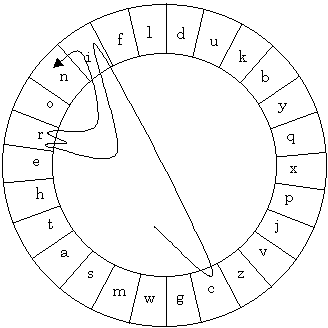
\includegraphics[scale=0.68]{Images/cirrin}
	\caption{Cirrin}
\end{figure}
\begin{figure}[h!]
	\centering
	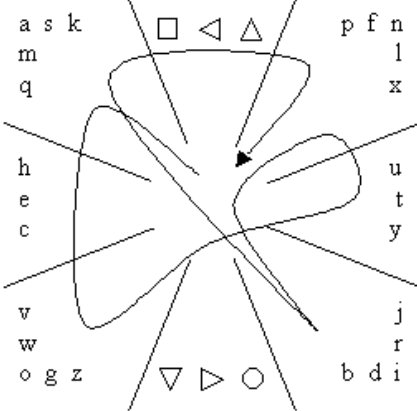
\includegraphics[scale=0.7]{Images/quickwriting.jpg}
	\caption{Quikwriting}
\end{figure}


\section{Traditional row layout based keyboards}
Qwerty was originally developed to reduce jamming in typewriters by placing letters in most common bi-grams far away from each other. But this problem is non-relevant to computer keyboards. Due to the popularity of Qwerty among all the existing typists, computer keyboards were also manufactured in Qwerty layout. Inherently, they were not optimized for comfortable typing. There were many alternative layouts created such as Dvorak, Colemak, Workman, Maltron, TypeMatrix etc. Some of them even have one handed layouts. Some gesture based keyboards like Gboard, SwiftKey also provide Dvorak, Colemak as options for layout on touchscreen. 

\begin{figure}[h!]
	\centering
	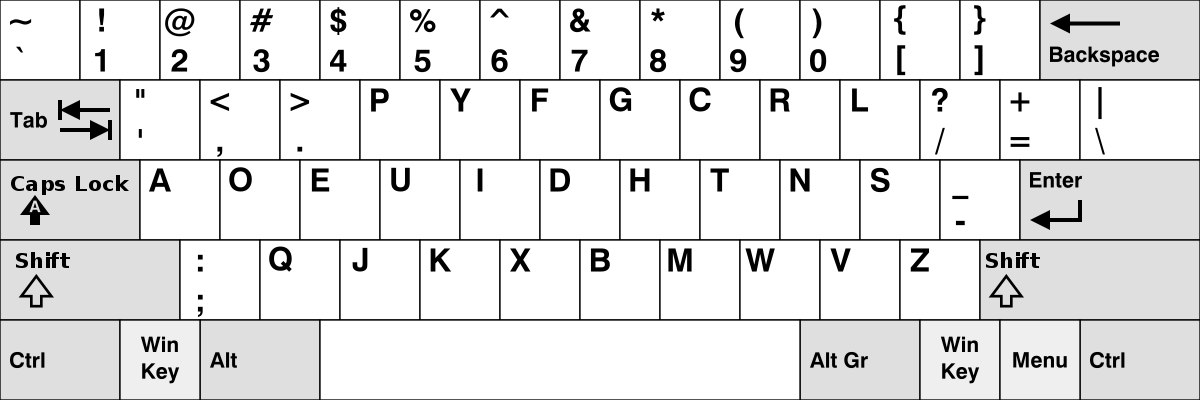
\includegraphics[scale=0.35]{Images/dvorak}
	\caption{Dvorak}
\end{figure}

\begin{figure}[h!]
	\centering
	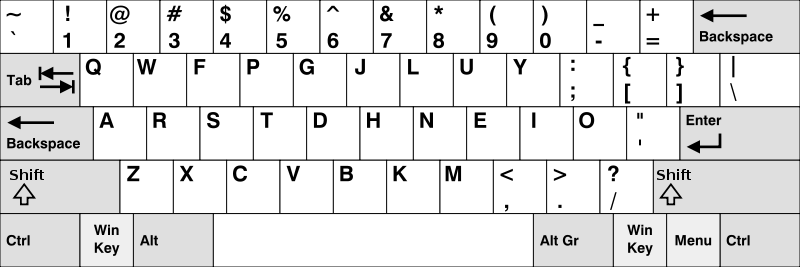
\includegraphics[scale=0.525]{Images/colemak}
	\caption{Colemak}
\end{figure}

\begin{figure}[h!]
	\centering
	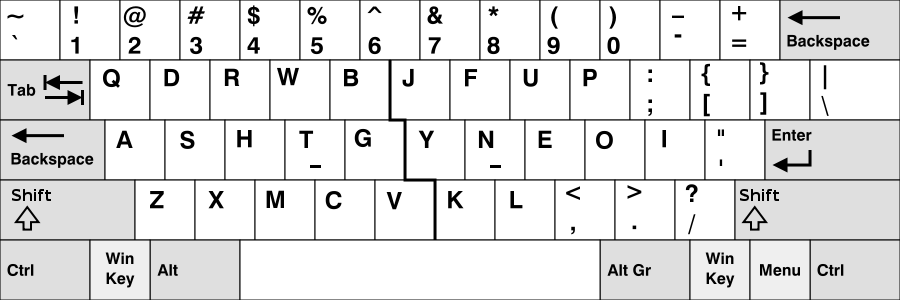
\includegraphics[scale=0.47]{Images/workman}
	\caption{Workman}
\end{figure}

\begin{figure}[h!]
	\centering
	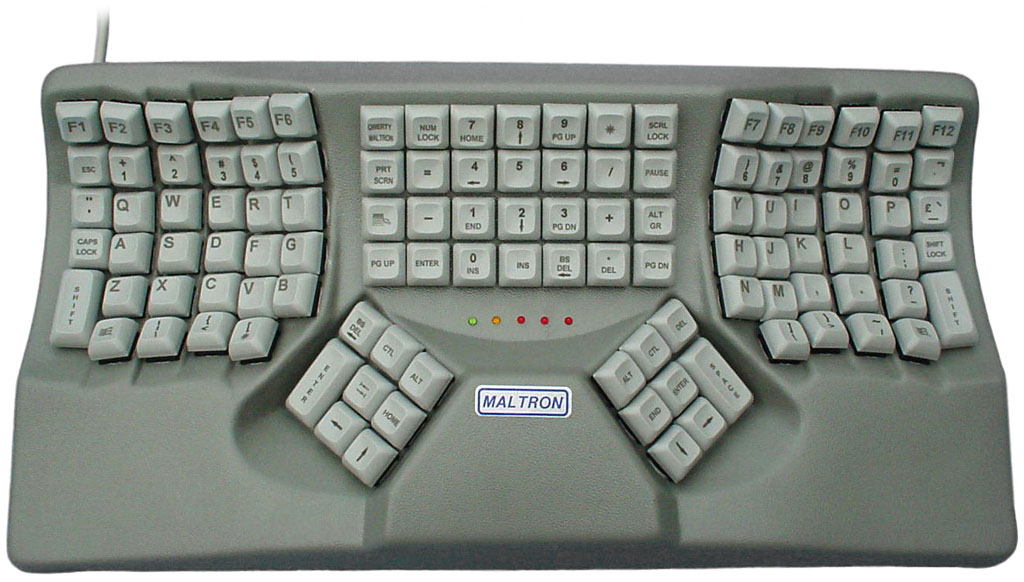
\includegraphics[scale=3.4]{Images/maltron}
	\caption{Maltron in Qwerty version}
\end{figure}

\begin{figure}[h!]
	\centering
	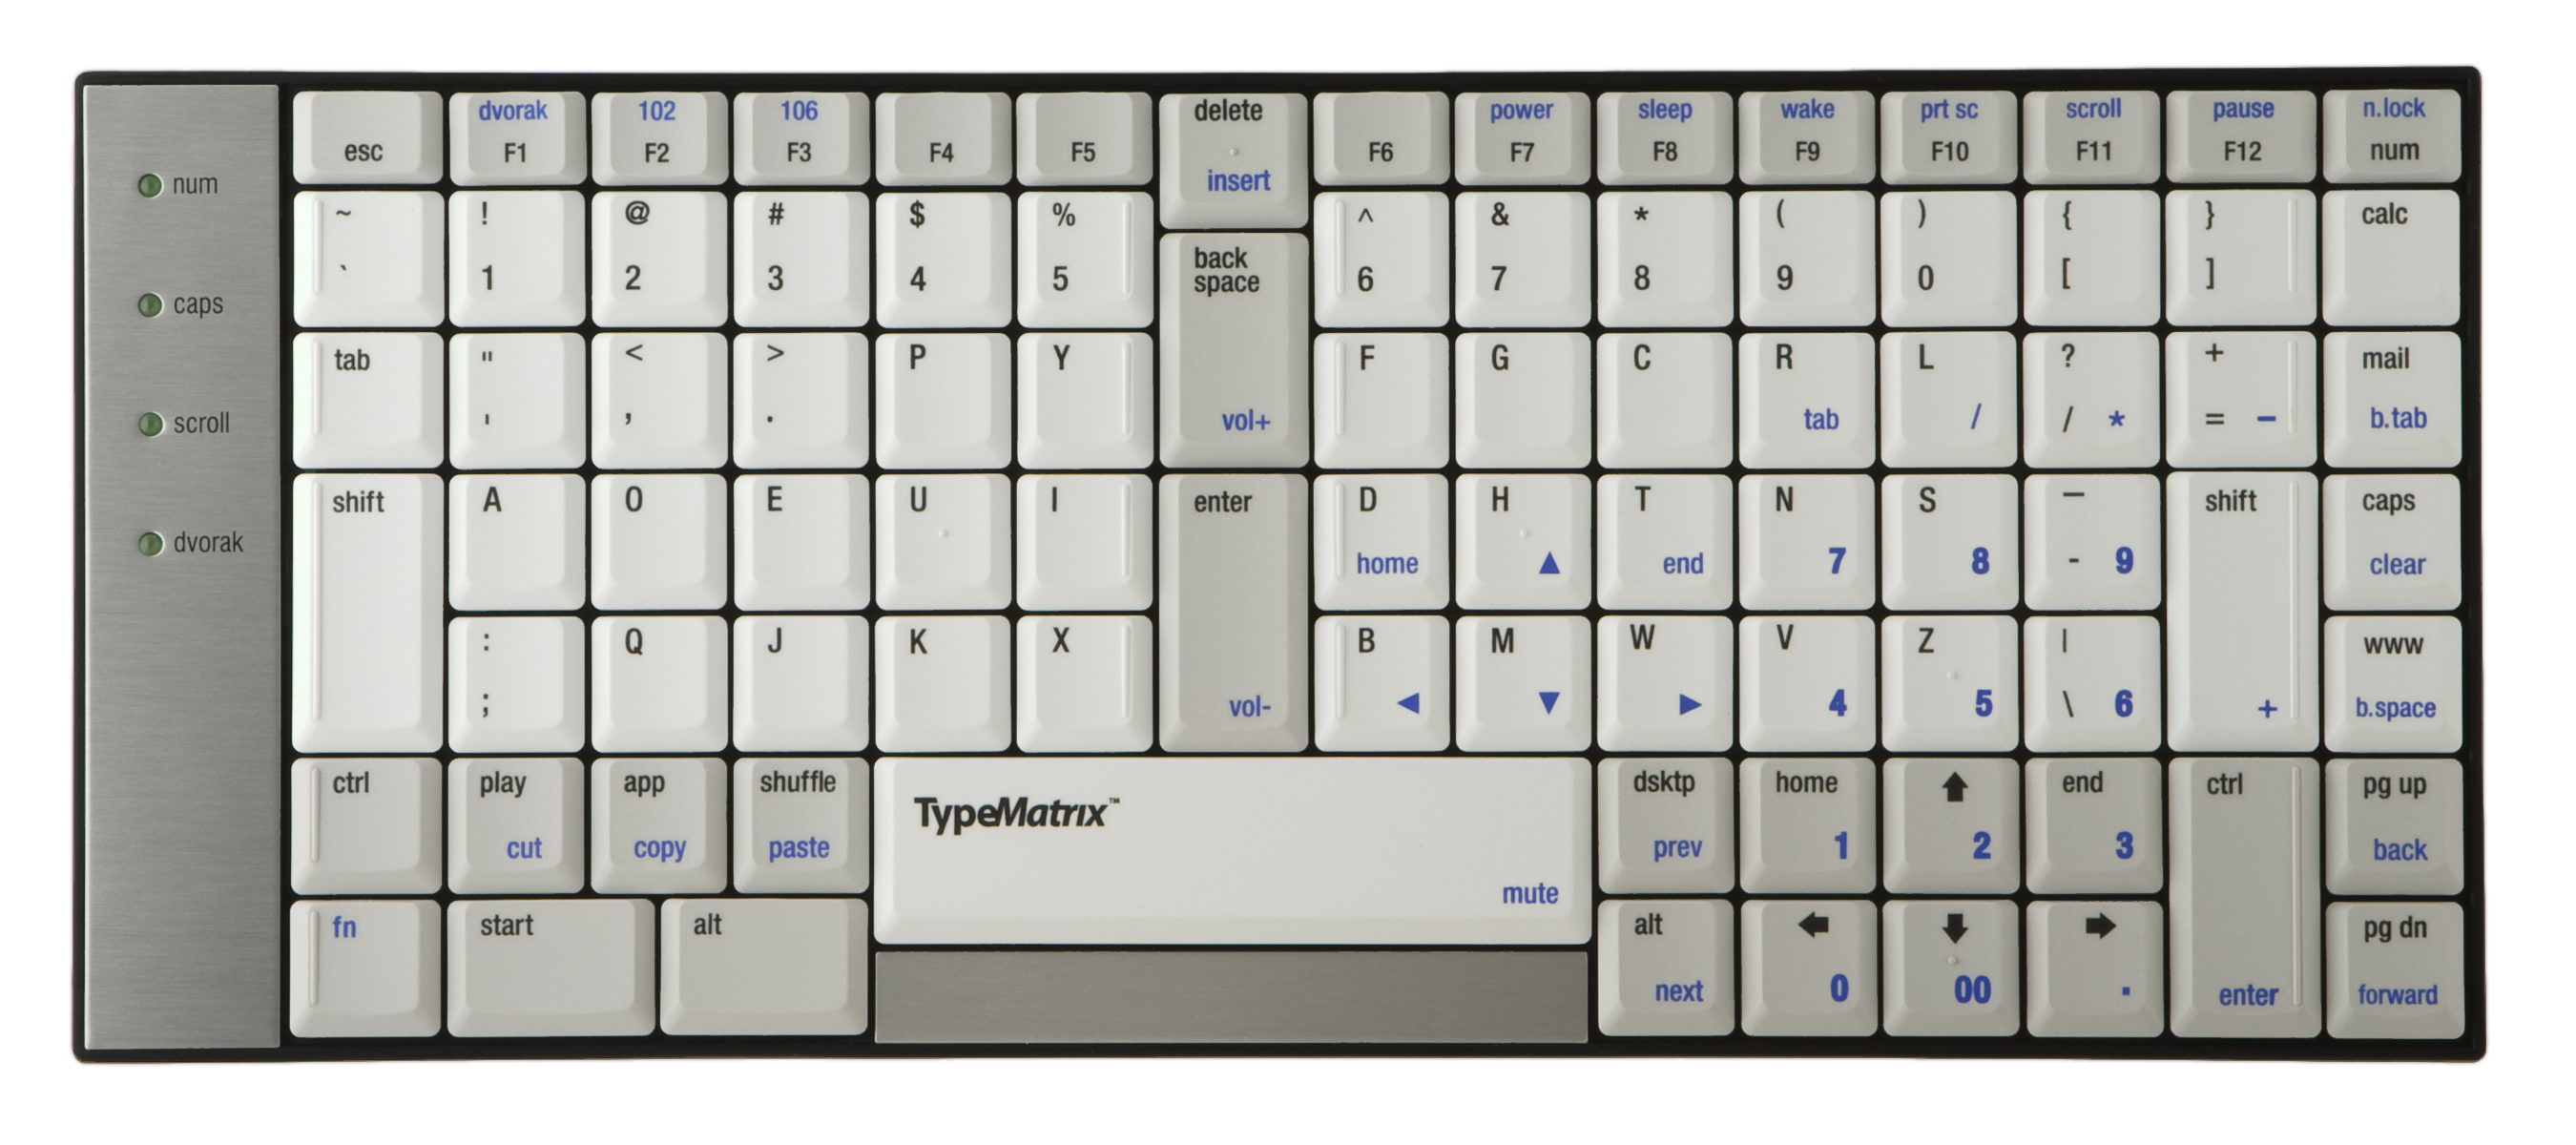
\includegraphics[scale=0.16]{Images/typematrix}
	\caption{TypeMatrix in Dvorak version}
\end{figure}

\begin{figure}[h!]
	\centering
	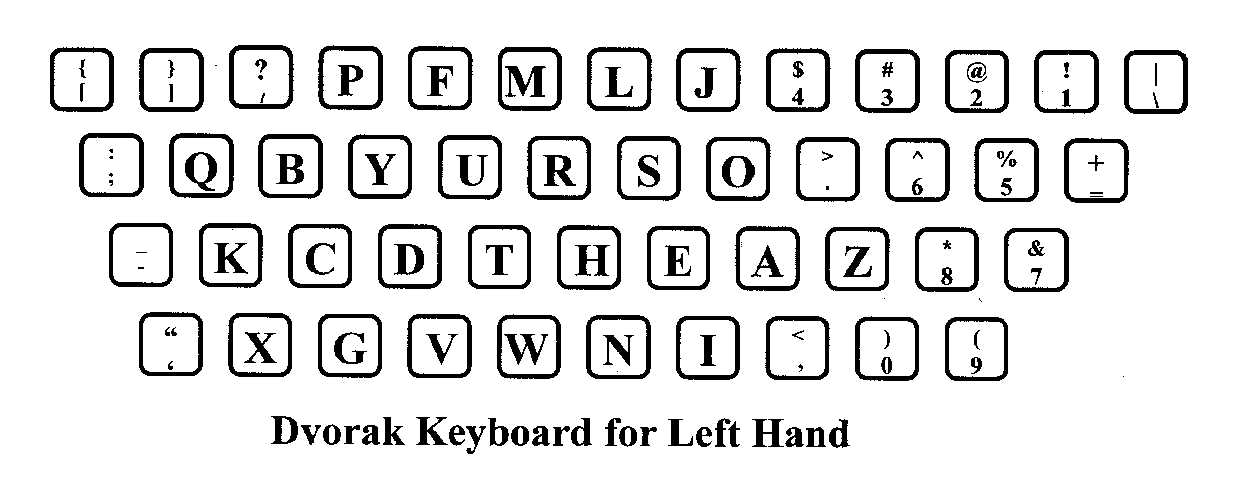
\includegraphics[scale=0.35]{Images/dvorak_left_hand}
	\caption{Left Handed Dvorak}
\end{figure}

\begin{figure}[h!]
	\centering
	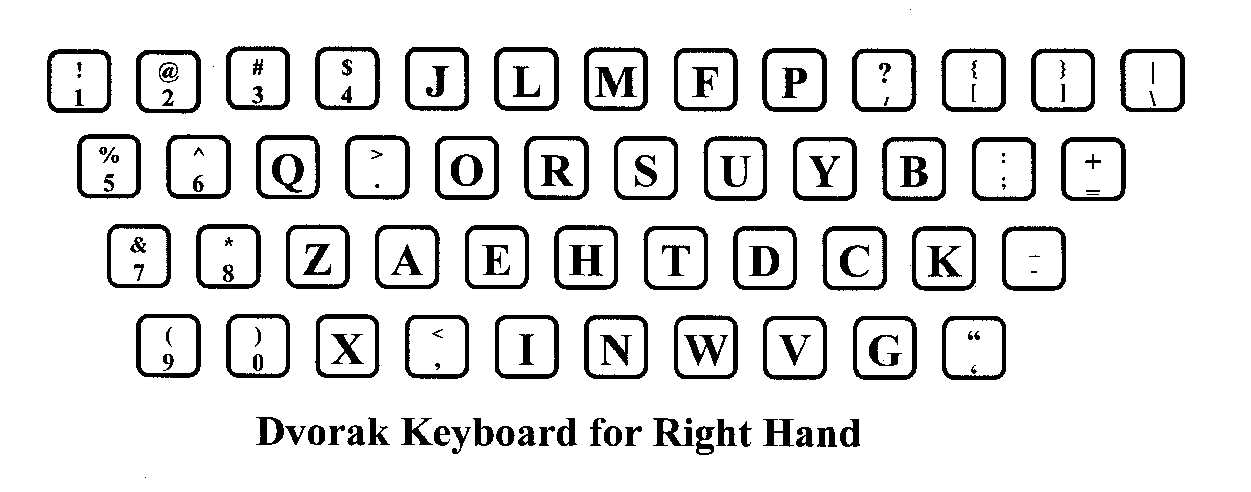
\includegraphics[scale=0.35]{Images/dvorak_right_hand}
	\caption{Right Handed Dvorak}
\end{figure}

However, it should be noted that although they are optimized for two handed typing using 8-10 fingers, they are not proven to be suitable for single finger gesture based typing. For example, Colemak is optimized mainly to retain AZXCV in their Qwerty positions to simplify clipboard operations. Dvorak is optimized to have all vowels on the left hand. These properties are undesirable in a gesture based keyboard. They exist primarily to help users use the same layout they use on their computers.


One of the most important problems with the usage of row layout based keyboards is that they create many gestures which have straight horizontal lines which results in many ambiguous and duplicate gestures. Hence the most effective solution would be to test the effect of slightly modified or staggered versions of existing keyboard layouts on the clarity and speed of gesture typing and to use the results to incrementally test and revise better keyboard layouts until we achieve the target speed and clarity.


\section{Existing Study on Gesture Optimized Keyboards}
Brian Smith, Xiaojun Bi, Shumin Zhai \citet{gesturerecog} have tried to tackle the problem and proposed 4 new keyboard layouts with different objectives as targets.

\begin{enumerate}
	
	\item GK-C: Clarity
	\item GK-S: Speed
	\item GK-D: Accuracy and Speed
	\item GK-T: Accuracy, Speed and Qwerty similarity
\end{enumerate}


\subsection{Procedure}
Since it is not possible to know how much weight needs to be given to each objective and also impossible to know what result to expect from the experiment, a dynamically adjustable technique needs to be employed. A technique called Pareto optimization had been successfully used in the past with good results. To do this, we find Pareto optimal set (Pareto front) of layouts in which none of its metric scores can be improved without hurting other scores. If there is a Pareto superior layout, it replaces all the other layouts it dominates. This process is repeated by iteratively changing the layout. At each iteration, two randomly chosen keys from previous iteration are swapped. This is repeated sufficient number of times to calculate a sufficiently large Pareto front. 

\begin{figure}[h!]
	\centering
	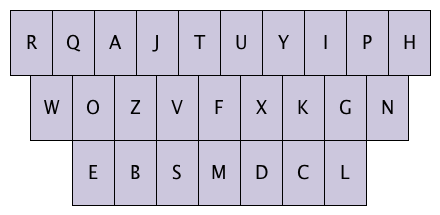
\includegraphics[scale=0.65]{Images/gkc}
	\caption{GK-C}
\end{figure}
\begin{figure}[h!]
	\centering
	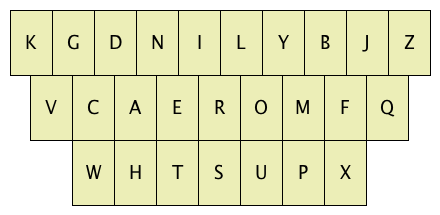
\includegraphics[scale=0.65]{Images/gks}
	\caption{GK-S}
\end{figure}
\begin{figure}[h!]
	\centering
	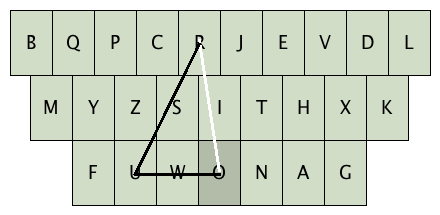
\includegraphics[scale=0.65]{Images/gkd}
	\caption{GK-D}
\end{figure}
\begin{figure}[h!]
	\centering
	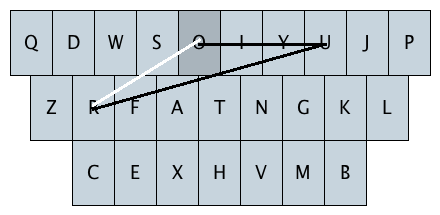
\includegraphics[scale=0.65]{Images/gkt}
	\caption{GK-T}
\end{figure}


\newpage
\subsection{Choosing the optimal layouts}
The Pareto optimal set is usually represented using a multidimensional graph. However, for the purpose of the main problem to be solved, we can take the 2D cross section of the graph which is as follows. The layouts with best metric in a parameter are given the value 1.0 for that metric and other layouts are normalized with respect to that metric.


\begin{figure}[h!]
	\centering
	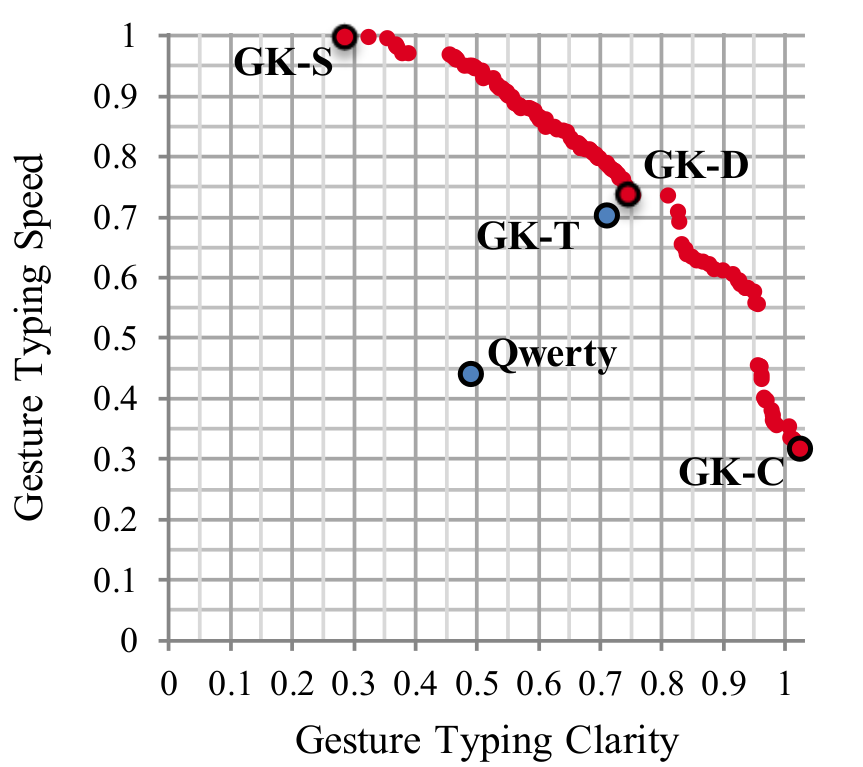
\includegraphics[scale=0.5]{Images/svc}
	\caption{2D Pareto Front [\cite{gesturerecog}]}
\end{figure}

Once we get the normalized graph, the 45 degree point on the 2D graph is taken as double optimized layout GK-D.
The triple optimized layout GK-T is taken as a layout that lies closest to the 45 degree line on the 3D graph of Pareto front.

\chapter{Layout Evaluation Metrics}
To evaluate the keyboard layouts, we use 3 weighted metrics. They are gesture clarity, gesture speed and qwerty similarity. Gesture clarity tells how well the layout is able to eliminate duplicate gestures for different words. Gesture speed tells how fast common words can be typed using gestures on the layout. Qwerty similarity tells how easy or difficult it is to learn the new layout for qwerty users.\\
These metrics are formulated as follow.
\section{Gesture Clarity}
The ideal trace of a word is a polyline connecting the midpoints of consecutive letters in the word. We find the ideal trace of each word. We also find the nearest neighbor of each word. This is the word which will most likely conflict with the original word. We take average of the distance between each word and its nearest neighbor for all the words weighted by word frequency. This is done using proportional shape matching.

The clarity is given by the average distance $d_{w}$ between each word and its nearest neighbor weighted by the word's frequency $f_{w}$ in a set of words L.
\begin{equation}Clarity=\sum_{w \in L} f_{w} d_{w}\end{equation}
\begin{equation} d_{w}= \min_{x \in L - \{w\} } d(w,x) \end{equation} 
\begin{equation} \sum_{w \in L } f_{w} = 1\end{equation}
We compute the distance between two ideal traces w and x via proportional shape matching. Each gesture is sampled into N equidistant points, and the distance is simply the average of the distance between corresponding points
\begin{equation}
d(w,x) = \frac{1}{N} \sum_{i=1}^{N} \| w_{i} - x_{i} \|_{2}
\end{equation}
For example, in our tests, the word "resistance" is the nearest neighbor of of the word "respective" and the distance between them is 9.11 units using this metric in Qwerty. 

\section{Gesture Speed}
Gestures are split into curves, line segments and corners and CLC model [\cite{strokes}] is used as the basis for this metric which in turn is based on human motor control theory. According to the CLC model, people tend to make faster strokes on longer line segments. The entry time for a stroke depends on the angle at a corner. However, this entry time much smaller than the entry time for a line segment irrespective of curve. Hence it can be easily ignored. 
\begin{equation} \label{eq:stroketime}
T( \overline{AB} )= m \cdot (\| \overline{AB} \|_{2})^n
\end{equation}
The total time required for the gesture can be simplified as the sum of times required by each segment and ignoring the small entry time of corners. 
\begin{equation} T(P)= \sum_{\overline{AB} \in P} T(\overline{AB}) \end{equation}
Time required by each segment can be pre-calculated based on bigrams and the average time per bigram can be calculated for the entire layout using bigram frequency weights.
\begin{equation} \label{eq:avgtimeperbigram} o(i-j)= \sum_{w \in L} f_{w} \cdot (\text {\# occurunces of i-j in w}) \end{equation}
To estimate the average time taken to complete a gesture we use \ref{eq:stroketime} and \ref{eq:avgtimeperbigram} with $K_{i}$ and $K_{j}$ as centres of i and j keys..
\begin{equation} G = \sum_{i,j \in \alpha} o(i-j) \cdot T(\overline{K_{i}K_{j}}) \end{equation}
To calculate speed, we divide the number of milliseconds in a minute by the average time taken.
\begin{equation}
Speed = \frac{60000}{G}
\end{equation}
For example, in our tests, the speed for the word "respective" using this metric in Qwerty is 4966.

\section{Qwerty Similarity}
The Qwerty similarity metric can be calculated using average of squared euclidean distances of keys from the the original Qwerty positions. However this metric is observed to punish farther placement of a small number of keys far more severely than a small displacement of multiple keys. Considering that keyboard is a grid, Manhattan distance was taken as a suitable metric to allow some infrequent keys to be moved more liberally without deeming the layout to be too dissimilar. To simplify Manhattan distance calculation, keys are aligned vertically by shifting middle row slightly to the left and bottom row to the right to align both of them to the top row.

The qwerty similarity is given by
\begin{equation}
Similarity = \sum_{i \in \alpha} (|k_{i_{x}}-q_{i_{x}}| + |k_{i_{y}}-q_{i_{y}}|)
\end{equation}
where i is a letter in alphabet,  $k_{i}$ is its position in new layout and $q_{i}$ is its position in qwerty layout in terms of (x,y) co-ordinates. For example, the position of key 'x' in iQwerty is (7,0) and in Qwerty, it is (8,1). Hence this key will contribute |7-8| + |0-1| = 2 units to the above sum as opposed to $\sqrt{2}$. 

\chapter{Existing Implementation}
The goal of this experiment is to find out the most optimal layouts in terms of clarity and speed while also taking into consideration the learning curve involved in adjusting to the layout for Qwerty users.
The implementation in the reference paper [\cite{gesturerecog}] is a three phase process. First, each metric is tested individually and normalized in order to make it easy to assign weightages. Next, Pareto optimization technique is used to find a set of optimal layouts called Pareto optimal layouts.

\section{Metric Normalization}
Tests are performed on each individual metric independently to estimate the maximum and minimum raw score for the metric.
10-30 optimizations are performed on each metric to achieve this.
Each optimization starts with a random keyboard layout and runs for 2000 iterations swapping two random keys at each iteration.
Simulated annealing is a probabilistic technique used to approximate the best solution when search space is too large and it is computationally expensive to explore all the possible solutions. This technique is used to keep better layouts with 100\% probability and other layouts with a fixed probability. It guarantees that better layouts are always kept in search space and some other layouts also get featured in search space with hopes that they too may lead to another optimal solution. This helps in escaping away from a local optimum and makes it possible to hopefully catch global optimum in case it is different from local maximum.
The normalized scores are used for the next phase.

\section{Pareto Front Initialization}
Using the technique used in Multi objective optimization of touchscreen keyboards, [\cite{weighting}] 22 different weightings are used for various linear combinations of metrics.
15 local neighborhood searches are performed. Each search is 2000 iterations.
The objective is to maximize the score of the linear combinations.
A Pareto optimal layout which is better than every other layouts in at least one metric each. The Pareto front is a set of Pareto optimal layouts which is initially empty but each additional Pareto optimal layout is added to the Pareto front as they are found. At the same time, any layout which ceases to be satisfy Pareto optimality condition is removed from the set. 

\section{Pareto Front Expansion}
200 passes are performed over the Pareto front to find Pareto optimal layouts similar to those in the Pareto front.
Performing initialization before this step ensures that all the possible solutions are reachable without swapping more than 2 keys at a time. This is because the Pareto front already contains a coarse approximation of optimal layouts and its expansion is carried out independently from every individual layout in the Pareto front to fine tune the results.

\section{Runtime}
For 40,000 words vocabulary, it took four machines with 32 threads each, three weeks to obtain the results.

\chapter{Proposed Changes in Metrics and Implementation}
After studying the existing approach towards generating optimal layouts, we examined various aspects individually to see whether we can get some improvements. We rationalized some of the possible changes and improvements and decided to test them using all the permutations of their combinations.

\section{Root level changes}
The existing layouts can be re designed with different number of rows or non linear arrangement of keys such as this layout called Interlaced Qwerty or iQwerty [\cite{iqwerty}]. This is a slight modification of original iQwerty proposal. The toggled middle row and quarter width extra alignment ensure that there are at most two characters in a straight diagonal trace. 

\begin{figure}[h!]
	\centering
	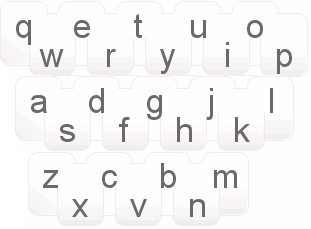
\includegraphics[scale=1]{Images/iqmod}
	\caption{Modified iQwerty}
\end{figure}


This layout reduces the number of linear duplicates significantly and contributes in both gesture clarity and speed. At the same time, it maintains Qwerty positions almost intact. Hence it can be used without incurring a significant learning curve.

\section{Metric changes}
We made some changes in each individual metric to make them resemble human gestures more closely.
\subsection{Gesture Clarity}
Calculating ideal trace as a series of straight line segments is not a realistic representative of human finger movements. Those can be better modeled using b-splines of appropriate order.
The proposed method is to generate a b-spline with n control points in the spline. One each at every character in the ideal trace. Each b-spline is split into 40 parts and point-wise distance from candidate trace at each split is recorded. Then we sum the distances of all 40 pairs and divide it by 40 to get the distance between the traces. We ignore all the words that start from a key farther than $\sqrt{2}$ units distance from the first letter of the candidate word and also those which end at a key farther than $\sqrt{2}$ units distance from the last letter. The word with the smallest distance from candidate word is the nearest neighbor Inverse of the weighted average distance of all nearest neighbors is the gesture clarity.

\subsection{Gesture Speed}
The existing method used bigram model which means character pairs like "th", "on", "er" etc. are used to represent strokes. Usage of bigram-only model gives a representation of only line segments. We can use a combination of bigrams, trigrams and quadgrams depending on the lengths of the words. Here trigrams, quadgrams are 3 and 4 consecutive characters respectively. We find them by splitting the words into parts of the size of the ngrams we are looking for. \\
e.g. If we split the word "thesis" into n grams, we will have "the", "hes", "esi" and "sis" as trigrams and quadgrams will be "thes", "hesi" and "esis" Such ngrams if more frequent - e.g. "the" - will represent the muscle memory involved in making the stroke, effectively making those strokes faster than other strokes with similar score in bigram-only metric.\\

Assuming that 'length' is the length of the trigram or quadgram, we use the following formula to calculate the time required.  [\cite{strokes}] 
\begin{equation}
time = 68.8 * length^{0.469} \end{equation}

\subsection{Qwerty Similarity}
There is a structural change in the layout. However, we can still use finer grid to find Manhattan distance and divide the result by the number of grid cells per character; in this case, 4 grid cells. The euclidean divisor here would be $4 \sqrt{2}$. In order to compare any proposed layout with another. We need to divide the similarity by this euclidean divisor in order to maintain parity.

\section{Implementation changes}
Our initial proposal was to use trigrams for small words, quadgrams for longer words, and pentagrams for very long words. However, later we decided to combine the benefits of trigrams and quadgrams and use them together.
Trigrams and Quadgrams are used for all words longer than 3 letters.
Quadgrams are designed to override trigrams in case of overlap.
The limits may be adjusted to include Pentagrams, Hexagrams etc. to represent gesture familiarity more accurately. However, due to low frequency of such ngrams in the corpus in hand, we decided to skip them for now.

We initially proposed Bezier curve as a representative of human gesture and used De-Casteljau's algorithm to divide the gesture trace into 20 equal parts. However, since a Bezier curve fails for longer word lengths, we switched to B-splines.
We use Cox-de-Boor algorithm [\cite{deboor}] to divide the gesture into 40 equal parts instead of using proportional shape matching. This allows us to use b-splines as gestures instead of straight lines.

The b-splines being used are of the order 2 and have additional points as midpoints of each bigram. These were added based on the observation that curve usually starts only in the second half of the gesture.

\chapter{Initialization and Testing Procedure}
For the the purpose of testing, we need a corpus which is composed of the letters which we have on our keyboard layouts. In our case, the layout is for English language. The experiment can accept any corpus and will give results corresponding to that corpus.

\section{Corpus Processing}
We use Brown corpus [\cite{brown}] as training data. It contains about 50,000 unique words.
We generate ngrams using top 5000 most frequent words.
Then we calculate ngram frequencies to find the most common ngrams to be used for optimization For the purpose of testing, we use top 100 ngrams. This is because the frequencies of ngrams reduce significantly beyond top 100 words and hence using them will not contribute significant advantage over not using them.

\section{Interface Quantization}
We use standard Qwerty keyboard layout and calculate key positions.
The centre of each key is considered as the key position.
The number of grid cells per key is multiplied by $\sqrt{2}$ to find the euclidean divisor of the layout.
We generate ideal trace for all the words. 
This information is used to calculate nearest neighbor and also the gesture time length.
We repeat this process for structural change in the keyboard. For modified iQwerty, we use a finer grid using 4 grid cells per key.

\subsection{Gesture Trace Evaluation}
We initially mapped traces of gestures using Bezier curves of order n where n is the word length. We also had evaluation method as whether this metric shows better result. We found that it was giving better results more than 90\% of the times up to 100\% for longer words but upon deeper investigation, we found two flaws in this method. One was that Bezier curve fails to represent longer words accurately. Another major flaw was that we did not use an ideal trace as a reference and only considered clearer and faster trace as an improvement. However, although more commonly true, it does not represent the real world scenario of human beings making the gestures. We found a better alternative to Bezier curve and chose b-splines. We also changed our testing methodology to check how many times the new trace is closer to ideal trace and not necessarily faster or clearer than old trace.
In the new method, the word gesture traces are interpreted as b-Splines. Our search space is the entire set of words except the current word. To prune the search space, the starting letter of the first control point is considered as unchanged and all the other traces are ignored. This is likely to be true because generally users choose the first character more precisely than rest of the characters in the stroke. Gesture entry time is expected to be directly proportional to Qwerty similarity. However, this assumption has not been tested since we are testing the metrics per layout basis instead of testing the layout optimality.

\chapter{Observations}
Distance between two b-splines is currently calculated using control points. Ideally we would need about 20 points to calculate distances with close to 90\% accuracy. To be able to propose new keyboard layout, we should consider 40 points in order to make more accurate predictions in approximately double the amount of time.

\begin{figure}[h!]
	\centering
	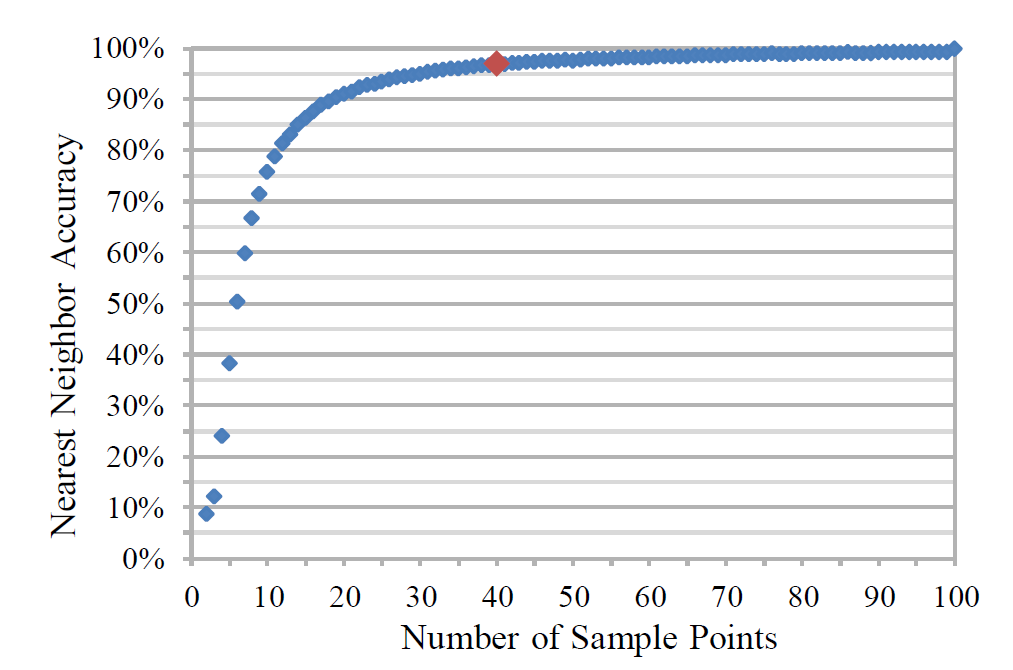
\includegraphics[scale=0.5]{Images/accuracy}
	\caption{Accuracy v/s Sample points }
\end{figure}

However, to prove the superiority of improved metrics over the older metrics, we performed distance and speed calculations for randomly chosen 100 words at a time with their own ideal traces. 100 words each were chosen from 4 to 10 letter words. Here, ideal trace is the b-spline of the order $2*n-1$ with $n-1$ additional points as midpoints of each bigram. Older metric uses straight lines connecting consecutive letters. Hence it creates a polyline with n points for a word of length n. The polyline goes through each character. New metric replaces common trigrams or quadgrams with b-splines. In case of trigram, we remove a pair of straight lines which represent that trigram and form a b-spline of the order 5 with 2 additional points as midpoints of each bigram in the trigram. In case of quadgram, we remove 3 straight lines that represent the quadgram and form o b-spline of order 7 with 3 additional points as midpoints of each bigram in the quadgram. 


\begin{figure}[h!] 
	\centering
	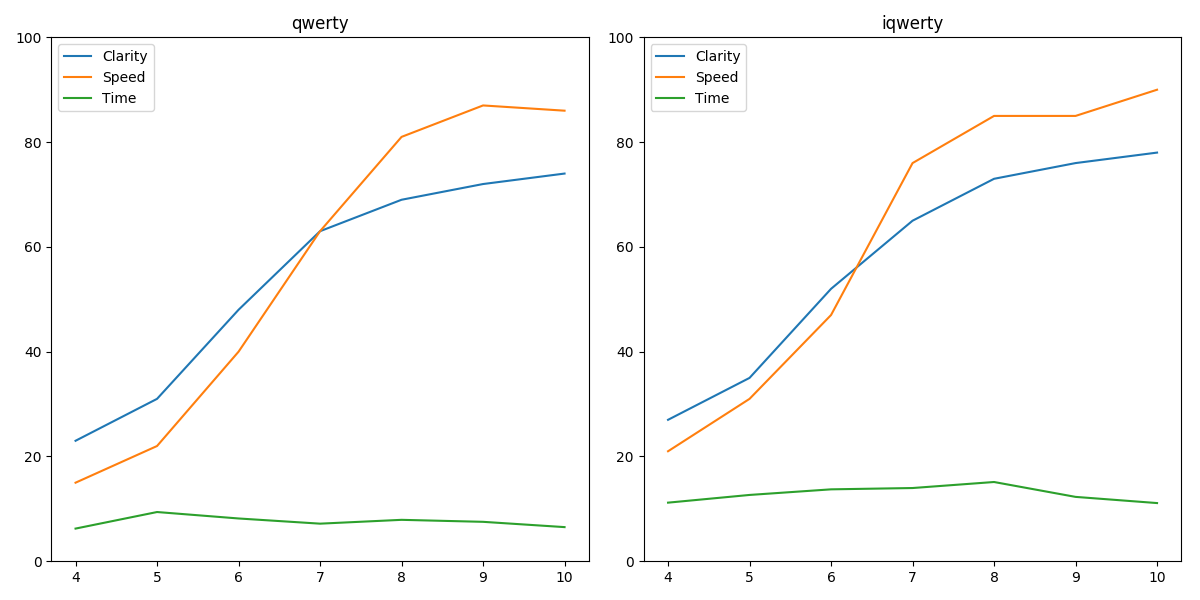
\includegraphics[scale=0.5]{Images/result}
	\caption{Results for Qwerty and iQwerty}
	\label{fig:results}
\end{figure}


The new metric is designed to fall back to old metric in case of non-availability of faster trace. Hence this metric guarantees that the new trace will not be worse. To measure the superiority, we calculate the percentage of times the metric gives results closer to ideal than old metric. In this case, we count the number of favorable cases from 100 samples each. Note that favorable cases or improvement in the metric refers to how close sampled cases are to their ideal metric counterpart and not necessarily faster or more accurate than older metric.


Figure \ref{fig:results} shows the results for experiments on Qwerty and iQwerty. The x-axis shows word-lengths The blue line indicates the percentage of times the new metric shows improvement over old metric in clarity and orange line shows the same for speed. The green line indicates the time taken in seconds to get both the results which was usually around 10 seconds in our tests and did not have any specific relation to word length. This is due to the fact that every word trace is converted to 40 parts and hence the evaluation should take the same time for every trace.  We see in the figure that both speed and clarity improvements are more prominent for longer words. The experiment was repeated multiple times and similar pattern was observed in general. The consistent positive improvements show that the use of new metrics can give more accurate representation of human gestures. This can help in getting more accurate results while evaluating alternative keyboard layouts.

\chapter{Conclusion}
We studied the possible shortcomings of an existing methodology for keyboard layout evaluation and brainstormed over how they an be overcome. We started experimentation with original metrics and proposed the use of ngram model instead of using only pairs of characters which is a bigram only model. We first experimented with ngrams of lengths 4 to 10 and found that their usage can represent human gestures more accurately more than 90\% of the times if we use Bezier curves to represent the portions of the word which contain the ngrams. We investigated further and found out that b-spline is a better alternative for longer words and hence we changed our procedure to use b-splines. We then used CLC model for speeds of words and proportional shape matching for clarity calculations using nearest neighbor of each word. We conducted both these experiments, clarity and speed calculation on two different layouts, 7 different word lengths, 100 random samples each.\\
The results confirm that our proposal shows improvement ranging from 20\% to 90\% due to the use of ngram model with results getting better for longer word lengths. Hence they also indicate that b-spline represents human gesture better than a Bezier curve or a polyline. We also showed that our metric design is also compatible with structural changes in Keyboard by running all the tests on iQwerty keyboard successfully.

\chapter{Future Work}
We have found that the proposed methodology gives better metrics than the earlier methodology. The results achieved so far can be used to propose new keyboard layouts and can have further refinements in stroke sampling and processing. The results can also be tested on users to check whether they follow the experimental assumptions about speed, clarity and familiarity. Pareto front calculation and expansion using new metrics will give more realistic results since the measured difference between ideal and improved metrics is smaller than that with old metrics. More refinements are possible with further understanding of advancements in human motor control.
Different types of usage patterns on social networks have resulted in newer paradigms. Patterns extracted from those can be incorporated into the metrics to be able to derive more optimal layouts or test entirely different keyboard structures.


\begin{singlespace}
%	\bibliographystyle{plain}
	\bibliography{refs}
\end{singlespace}

\end{document}
